\documentclass[11pt]{article}
%\usepackage{fullpage}
\usepackage[top=2cm, bottom=1.5cm, left=1.5cm, right=1.5cm]{geometry}
\usepackage{amsmath,amsthm,amsfonts,amssymb,amscd}
\usepackage{xcolor}
\usepackage{graphicx}
\usepackage[utf8]{inputenc}
\usepackage[english]{babel}
\usepackage{fancyhdr}
\usepackage{wrapfig}

\pagestyle{fancy}
\fancyhf{}
\fancyhead[LO]{Mechanics \& Relativity F3210}
\fancyhead[RO]{Workshop 8: Gravitation}
%\fancyfoot[CE,CO]{\leftmark}
%\fancyfoot[LE,RO]{\thepage}

%answers
\usepackage{etoolbox}
\providetoggle{answers}
\settoggle{answers}{false}

\newcommand\vect[1]{\underline{\mathbf{#1}}}
\newcommand\unitvect[1]{\hat{\boldsymbol{#1}}}

\begin{document}

\noindent
\textbf{\textcolor{red}{Please upload your solution to Problem 3 to canvas for marking after the workshop.}}\\

\section*{Problem 1}

The radius $R_h$ and mass $M_h$ of a black hole are related by $R_h = 2GM_h / c^2$, where $c$ is the speed of light. Assume that the gravitational acceleration $a_g$ of an object at a distance $r_o = 1.001R_h$ from the centre of a black hole is given by $a_g = GM / r^2$ (it is, for large black holes). \\
(a) In terms of $M_h$, find $a_g$ at $r_o$. \\
(b) If an astronaut of height 1.70 m is at $r_o$ with her feet down, what is the difference in gravitational acceleration between her head and feet? \\



\noindent

\section*{Problem 2}

Zero, a hypothetical planet, has a mass of $5.0 \times10^{23}$ kg, a radius of $3.0 \times 10^6$ m, and no atmosphere. A 10~kg space probe is to be launched vertically from its surface. If the probe is launched with an initial energy of $5.0 \times 10^7$ J, what will be its kinetic energy when it is $4.0 \times 10^6$ m from the centre of Zero?\\


\section*{\textcolor{red}{Problem 3}}
\fbox{\begin{minipage}{\textwidth}
Observations of the light from a certain star indicate that it is part of a binary (two-star) system. This visible star has orbital speed $v = 270$ kms$^{-1}$, orbital period $T = 1.70$ days, and approximate mass $m_1 = 6M_s$, where $M_s$ is the Sun's mass, $1.99 \times 10^{30}$ kg. Assume that the visible star and its companion star, which is dark and unseen, are both in circular orbits, as in the figure shown below. What integer multiple of $M_s$ gives the approximate mass $m_2$ of the dark star?

\end{minipage}}

\begin{figure}[h]
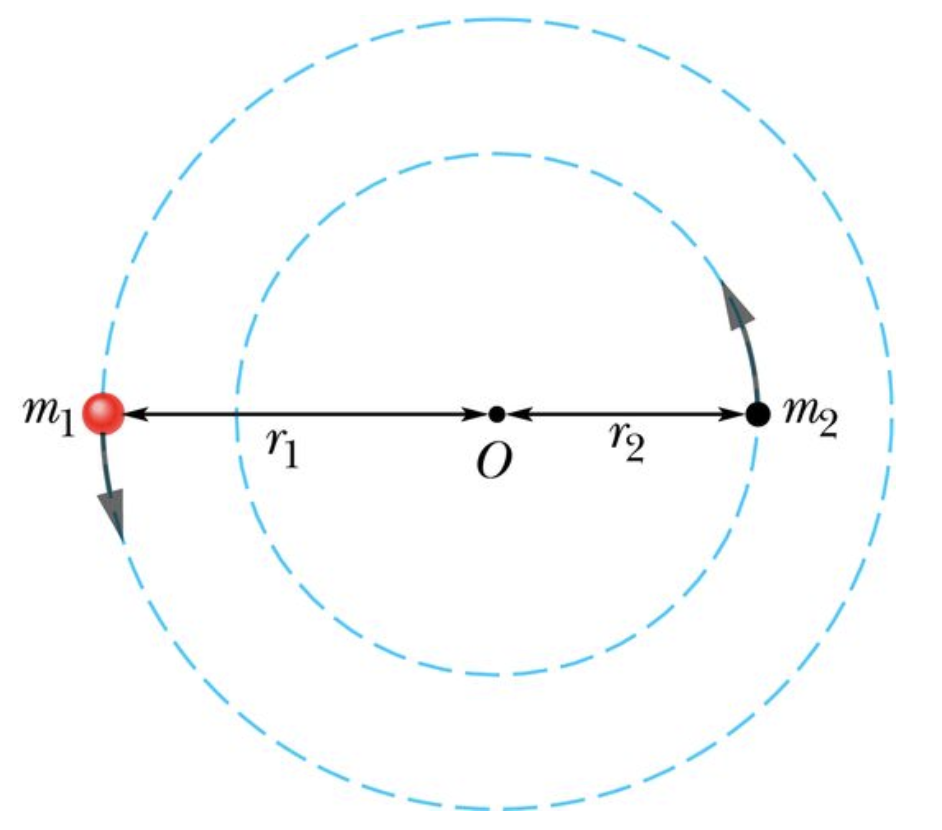
\includegraphics[scale=0.25]{2021-W8-Q3}

\end{figure}

\section*{Problem 4}

A satellite orbits a planet of unknown mass in a circle of radius $2.0 \times 10^7$ m. The magnitude of the gravitational force on the satellite from the planet is $F = 80$ N.  What is the kinetic energy of the satellite in this orbit?\\

%\vspace{0.5cm}
\section*{Want more practice?}
\small
Further problems on Newton's Gravitation: Chapter 13.1-13.3 \\
Further problems on Gravitational PE: Chapter 13.4-13.5 \\
Further problems on Kepler's Laws \& Orbits: Chapter 13.6-13.7 \\
\end{document}





 




 


